\documentclass[tikz,border=8pt]{standalone}
\usepackage{amsmath,amssymb}
\usetikzlibrary{arrows.meta,automata,positioning,quotes}
\begin{document}
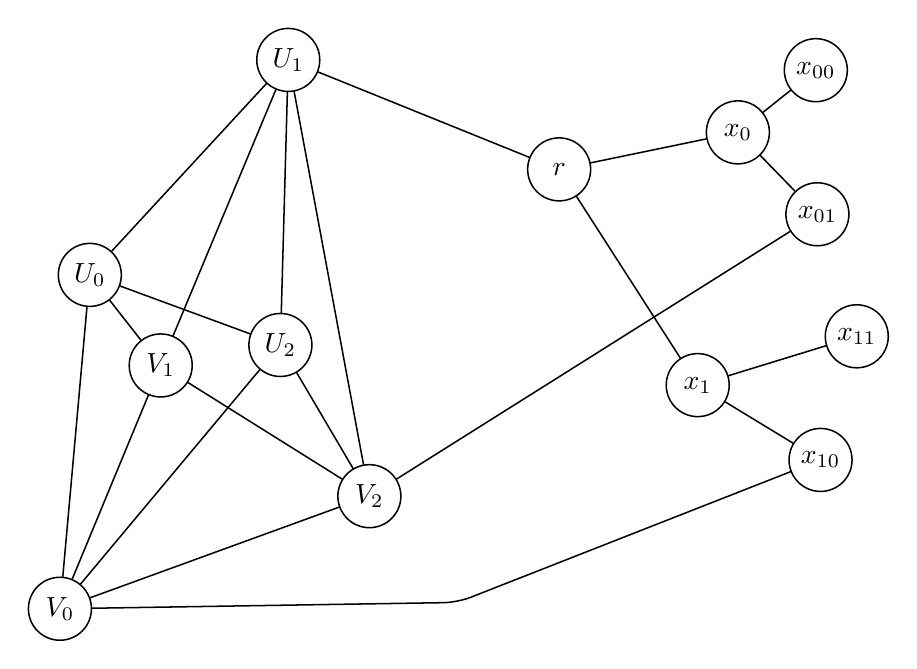
\begin{tikzpicture}[x=1cm,y=1cm]
\tikzset{
  graphnode/.style={circle,draw=black,line width=0.55pt,minimum size=8mm,inner sep=1pt,font=\sffamily},
  graphedge/.style={draw=black,line width=0.55pt,line cap=round,line join=round},
  directed/.style={graphedge,-{Stealth[length=2.4mm,width=2.0mm]}},
  undirected/.style={graphedge}
}
\node[graphnode] (n_U0) at (-5.99,0.98) {$U_0$};
\node[graphnode] (n_U1) at (-3.47,3.71) {$U_1$};
\node[graphnode] (n_U2) at (-3.57,0.09) {$U_2$};
\node[graphnode] (n_V0) at (-6.37,-3.26) {$V_0$};
\node[graphnode] (n_V1) at (-5.09,-0.17) {$V_1$};
\node[graphnode] (n_V2) at (-2.44,-1.83) {$V_2$};
\node[graphnode] (n_r) at (-0.03,2.32) {$r$};
\node[graphnode] (n_x0) at (2.24,2.79) {$x_0$};
\node[graphnode] (n_x1) at (1.73,-0.42) {$x_1$};
\node[graphnode] (n_x00) at (3.23,3.58) {$x_{00}$};
\node[graphnode] (n_x01) at (3.25,1.75) {$x_{01}$};
\node[graphnode] (n_x10) at (3.29,-1.37) {$x_{10}$};
\node[graphnode] (n_x11) at (3.75,0.20) {$x_{11}$};
\draw[undirected] (n_U0) -- (n_U1);
\draw[undirected] (n_U1) -- (n_U2);
\draw[undirected] (n_U0) -- (n_U2);
\draw[undirected] (n_V0) -- (n_V1);
\draw[undirected] (n_V1) -- (n_V2);
\draw[undirected] (n_V0) -- (n_V2);
\draw[undirected] (n_U0) -- (n_V0);
\draw[undirected] (n_U1) -- (n_V1);
\draw[undirected] (n_U2) -- (n_V2);
\draw[undirected] (n_U0) -- (n_V1);
\draw[undirected] (n_U1) -- (n_V2);
\draw[undirected] (n_U2) -- (n_V0);
\draw[undirected] (n_U1) -- (n_r);
\draw[undirected] (n_r) -- (n_x0);
\draw[undirected] (n_r) -- (n_x1);
\draw[undirected] (n_x0) -- (n_x00);
\draw[undirected] (n_x0) -- (n_x01);
\draw[undirected] (n_x1) -- (n_x10);
\draw[undirected] (n_x1) -- (n_x11);
\draw[undirected] (n_x01) -- (n_V2);
\draw[undirected,rounded corners=5pt] (n_x10) -- (-1.32,-3.18) -- (n_V0);
\end{tikzpicture}
\end{document}
